\section{Results and Discussion}

%How complete is our model so far? What can we model? How big are the uncertainties?
%
%What where the models and approaches that performed the best? \dots for each sector:
%Which sectors were most important (biggest fraction of emissions)

With indicators for all sectors, we can now model how the \co emissions for each of the eight countries behaved for the first half of 2020. For that, we combine all sectors for each country according to each sector's contribution.


We provide our result in \autoref{fig:predictedCO2}. The data is seasonality adjusted already, which means that the height of each line directly gives the fraction of \co emissions we would have expected for this month. This is our main result for this Milestone and it completely meets our expectations. We took a lot of different data into account and tried to model \co emissions as accurately as possible with our (limited) resources. Since we took so many different data sets into consideration we think it is fair to assume that we minimized the overall uncertainty. We used a lot of different machine learning models, each one carefully chosen such that we obtain the best results only. 

We still think that we could have done even better with more resources but nevertheless, we are very satisfied with the outcomes of our model so far. We therefore conclude that our model and approach is valid, delivering a result with which we can finally compare COVID-19 case numbers now. This will be done in the next and final Milestone.

\begin{figure}[hb!]
	\centering
	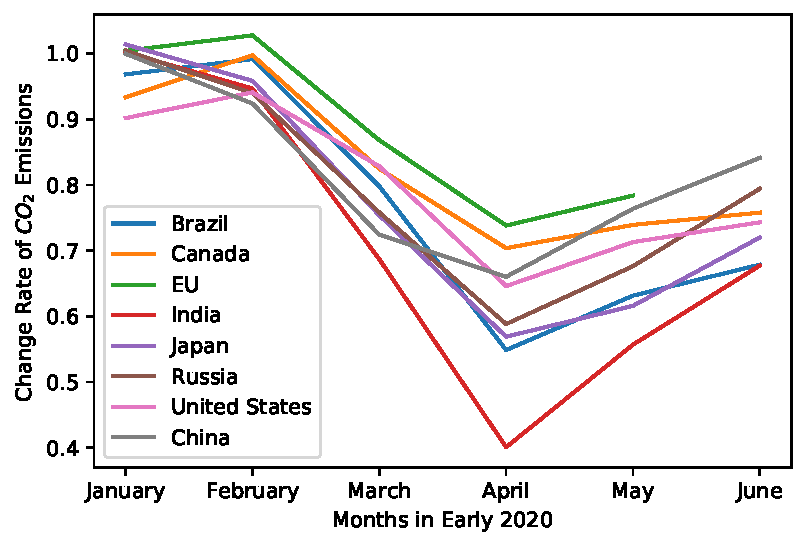
\includegraphics[width=0.7\linewidth]{../predictions/change_rate.pdf}
	\caption{Change of CO2 emissions for each country we consider. As expected, we observe a drop in \co emissions.}
	\label{fig:predictedCO2}
\end{figure}


%\begin{itemize}
%	\item \textbf{Transport:}
%	\item \textbf{International Aviation/Shipping:}
%	\item \textbf{Buildings:}
%	\item \textbf{Other industrial combustion:}
%	\item \textbf{Other sectors:}
%	\item \textbf{Power industry:}
%\end{itemize}